% ---------------------------------------------------------------------------
\section{Question 1 -- What does a sum remember?}
All numerical claims below are verified by brute force in Part Q1 of the notebook.

\subsection*{(a) Affine message}
With $\phi(x)=wx+c$,
\[
  \sum_{u\in N(v)}\phi(x_u)=\sum_{u\in N(v)}(wx_u+c)=w\,S_v+c\,n_v ,
  \qquad h_v=\rho\big(wS_v+c\,n_v\big).
\]
The aggregated message is a function of the pair $(n_v,S_v)$ only, and $\rho$ sees nothing else. Hence two
neighbourhoods with the same $n_v$ and $S_v$ produce the \emph{same} input to $\rho$ and therefore the same
$h_v$, whatever $w$, $c$ and $\rho$ are. Example: $N_1=\{-1,+1,0\}$ and $N_2=\{0,0,0\}$ both have
$n_v=3$, $S_v=0$, but contain one and three steady neighbours respectively. Because a slowing and a speeding-up
neighbour cancel in $S_v$, the affine layer cannot tell ``one slowing + one speeding'' from ``two steady''. The
notebook confirms identical outputs for random $(w,c)$ and a nonlinear $\rho$.

\subsection*{(b) A nonlinear scalar message that stores all three counts}
Let $n_-,n_0,n_+$ be the numbers of slowing, steady and speeding-up neighbours, with
$1\le n_-+n_0+n_+\le K$. Each count is at most $K$, i.e.\ a digit in base $B=K+1$. Choose
\[
  \phi(-1)=1,\qquad \phi(0)=K+1,\qquad \phi(+1)=(K+1)^2 .
\]
Then $s=\sum_{u}\phi(x_u)=n_-+n_0(K+1)+n_+(K+1)^2$, which is exactly the base-$(K+1)$ number with digits
$(n_+,n_0,n_-)$. Because every digit is $\le K<K+1$, no carry can occur, so the representation is unique.
Decoding:
\[
  n_-=s \bmod (K+1),\qquad n_0=\Big\lfloor \tfrac{s}{K+1}\Big\rfloor \bmod (K+1),\qquad
  n_+=\Big\lfloor \tfrac{s}{(K+1)^2}\Big\rfloor .
\]
A smaller base fails: with base $K$, $K$ slowing neighbours give $s=K=\phi(0)$, the same as one steady neighbour.
For $K=8$ ($B=9$, $\phi=(1,9,81)$) the notebook enumerates all $164$ count triples with $1\le$ total $\le 8$, builds
every neighbourhood, sums the messages and checks that (i) all $164$ sums are distinct and (ii) the decoder
recovers every triple exactly. Both checks pass; e.g.\ $(n_-,n_0,n_+)=(2,1,3)\mapsto 2+9+243=254$.

\emph{Counting non-steady neighbours.} Take $\phi(x)=x^2$ (equivalently $|x|$): $\phi(\pm1)=1$, $\phi(0)=0$,
so $\sum_u\phi(x_u)=n_-+n_+$ for any neighbourhood size (also verified).

\subsection*{(c) Sum, mean and max with one-hot messages}
Write the aggregated vectors as $\mathbf s=(n_-,n_0,n_+)$ (sum), $\mathbf m=\mathbf s/n$ (mean) and
$\mathbf M=(\mathbb 1[n_->0],\mathbb 1[n_0>0],\mathbb 1[n_+>0])$ (max). The table was also confirmed by
enumerating all $164$ neighbourhoods of size 1--8 and searching for collisions.

\begin{center}
\small
\begin{tabular}{p{3.0cm}lcp{8.6cm}}
\toprule
Task & Method & Possible? & Reason \\
\midrule
(i) Count steady & Sum & Yes & $\rho$ reads coordinate 2: $n_0=s_2$. \\
 & Mean & No & $\{0\}$ and $\{0,0\}$ both give $\mathbf m=(0,1,0)$; answers $1$ vs $2$. \\
 & Max & No & $\{0\}$ and $\{0,0\}$ both give $\mathbf M=(0,1,0)$; answers $1$ vs $2$. \\
\midrule
(ii) More than half slowing & Sum & Yes & $n=s_1+s_2+s_3$; answer $=\mathbb 1[s_1>s_2+s_3]$ (i.e.\ $2s_1>n$). \\
 & Mean & Yes & coordinate 1 is the fraction slowing: answer $=\mathbb 1[m_1>\tfrac12]$. \\
 & Max & No & $\{-1,0\}$ and $\{-1,-1,0\}$ both give $\mathbf M=(1,1,0)$; answers No ($1/2$) vs Yes ($2/3$). \\
\midrule
(iii) Any slowing & Sum & Yes & answer $=\mathbb 1[s_1>0]$. \\
 & Mean & Yes & answer $=\mathbb 1[m_1>0]$ (since $m_1=n_-/n$ and $n\ge1$). \\
 & Max & Yes & answer $=M_1$. \\
\bottomrule
\end{tabular}
\end{center}
Sum is the most expressive aggregator (it keeps the multiset counts), mean keeps only proportions (loses $n$),
and max keeps only which trends are present (loses multiplicities), which is why it still detects ``any''.

% ---------------------------------------------------------------------------
\section{Question 2 -- Which way is the slowdown moving?}

\subsection*{(a)(i) Least-squares fit of the symmetric layer}
With $x_{20}(t)=1$ and all other readings 0, the only nonzero predictions are
$\hat x_{19}=b$, $\hat x_{20}=a$, $\hat x_{21}=b$, while the correct next snapshot is
$x_{19}=1$, $x_{20}=0$, $x_{21}=0$. Hence
\[
  L(a,b)=(b-1)^2+a^2+b^2,\qquad
  \frac{\partial L}{\partial a}=2a=0,\qquad \frac{\partial L}{\partial b}=2(b-1)+2b=0
  \;\Rightarrow\; a=0,\; b=\tfrac12,\; L_{\min}=\tfrac12 .
\]
Sensors 19 and 21 receive identical inputs (one neighbour equal to 1), so they must receive the same
prediction; the best compromise splits the slowdown equally. \texttt{np.linalg.lstsq} returns the same
$a=0,\ b=0.5$, SSE $=0.5$.

\subsection*{(a)(ii) Rolling the fitted layer forward}
Figure~\ref{fig:q2} shows the true motion and the 20-step autoregressive roll-out of $\hat x_i(t+1)=\tfrac12(x_{i-1}+x_{i+1})$
on the bump $x_i(0)=e^{-(i-20)^2/8}$ (same colour scale). The true bump translates one sensor per step without changing shape (its peak
reaches sensor 0 at $t=20$ and wraps round the ring). The symmetric layer never moves the bump: its peak stays at
sensor 20 while it spreads out and flattens (peak $1\to\approx0.40$ at $t=20$, total mass conserved). It
is a diffusion operator rather than a transport operator.

\begin{figure}[h]
  \centering
  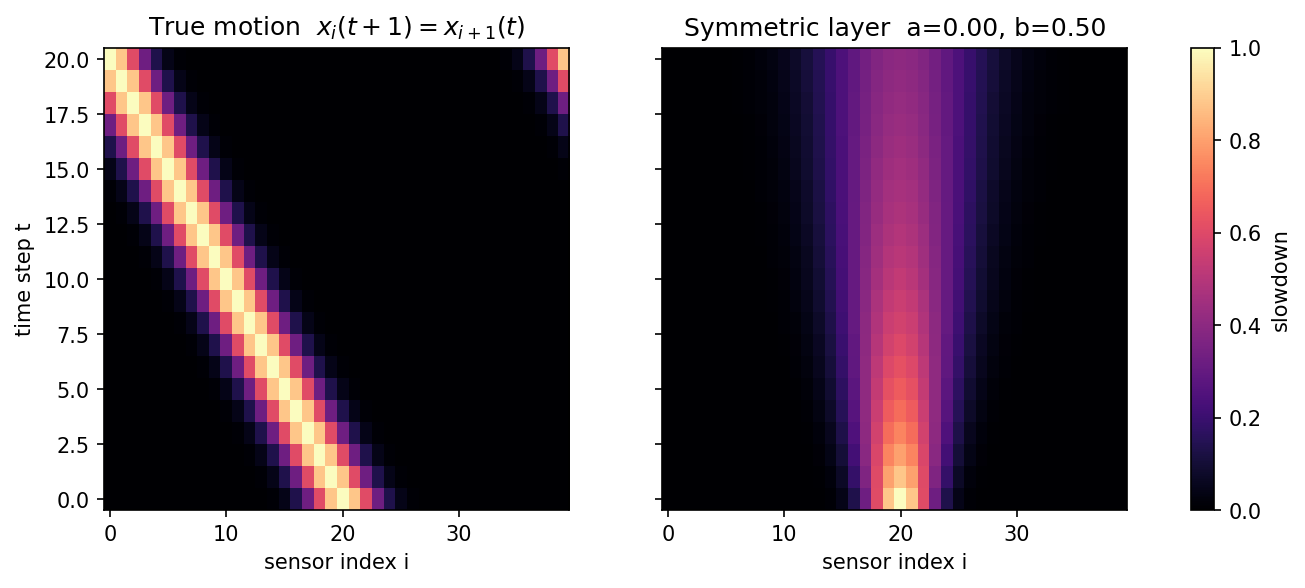
\includegraphics[width=0.82\linewidth]{figures/q2a_heatmaps.png}
  \caption{Q2(a)(ii): true backward motion (left) versus the fitted symmetric layer applied recursively (right).}
  \label{fig:q2}
\end{figure}

\subsection*{(b) Direction-aware weights}
Choose $a=0,\ w_-=0,\ w_+=1$. Substituting,
$\hat x_i(t+1)=0\cdot x_i(t)+0\cdot x_{i-1}(t)+1\cdot x_{i+1}(t)=x_{i+1}(t)=x_i(t+1)$ for every input and
every $i$ (indices mod 40), so the prediction is exact. Because the layer now knows which neighbour is
\emph{ahead} and which is \emph{behind}, the mirror symmetry $i\mapsto 40-i$ that forced $\hat x_{19}=\hat x_{21}$ in
(a) is broken. The layer can copy from the ahead neighbour only, which is exactly the motion rule.

\emph{As a 1-D convolution.} In PyTorch-style cross-correlation, the kernel entries that multiply
$[x_{i-1},x_i,x_{i+1}]$ are $[w_-,a,w_+]=[0,0,1]$. The ring is handled with \textbf{circular padding} of one
sensor on each side (\texttt{F.pad(x,(1,1),mode="circular")}, or \texttt{padding\_mode="circular"} in
\texttt{nn.Conv1d}), so sensor 39 sees sensor 0 as its ahead neighbour. The notebook confirms that this
convolution equals \texttt{np.roll(x,-1)} on random inputs.

\subsection*{(c) History with equal neighbour weights}
\textbf{(i) Backward motion.} The rule $x_i(t)=x_{i+1}(t-1)$ gives $x_{i-1}(t)=x_i(t-1)$: the reading that was at
sensor $i$ has moved to sensor $i-1$. The target is $x_i(t+1)=x_{i+1}(t)$. Choose $a=0,\ b=1,\ c=-1$:
\[
  \hat x_i(t+1)=x_{i-1}(t)+x_{i+1}(t)-x_i(t-1)=x_{i-1}(t)+x_{i+1}(t)-x_{i-1}(t)=x_{i+1}(t)=x_i(t+1). \checkmark
\]
\textbf{(ii) Forward motion} $x_i(t+1)=x_{i-1}(t)$. Now $x_i(t-1)=x_{i+1}(t)$ (the old reading at $i$ moved
forward to $i+1$), and with the same coefficients
\[
  \hat x_i(t+1)=x_{i-1}(t)+x_{i+1}(t)-x_i(t-1)=x_{i-1}(t)+x_{i+1}(t)-x_{i+1}(t)=x_{i-1}(t)=x_i(t+1). \checkmark
\]
The same coefficients are exact for both directions; the notebook checks both on 200 random patterns
(maximum error $4\times10^{-16}$).

\textbf{(iii) Why history helps.} The previous reading $x_i(t-1)$ equals the current reading of whichever
neighbour the pattern has just moved \emph{into}, i.e.\ the neighbour that holds information which has already
passed sensor $i$. Subtracting it cancels that neighbour from the symmetric sum and leaves the neighbour whose
reading is about to arrive. The direction is therefore read from the data (the pair
$(\mathbf x(t-1),\mathbf x(t))$ encodes the velocity), not from asymmetric weights. In effect the layer is the
leapfrog discretisation of the wave equation, $x(t+1)-2x(t)+x(t-1)=x_{i+1}-2x_i+x_{i-1}$, whose solutions move
in either direction depending on the initial velocity. For traffic models this means temporal context can
supply directional information that an undirected graph convolution alone cannot.
